\section{Nõuete defineerimine}
\label{chapters:analysis_requirements}
\subsection{Funktsionaalsed nõuded}
\label{subsec_func_req}
Funktsionaalsete nõuete määramisel lähtutakse erinevate osapoolte vajadusest - süsteemi kasutaja ja süsteemi 
administraator. Nõuete sõnastamisel on aluseks töö autori isiklik kogemus ja teadmised sihtgrupi vajadustest ja nõuetest.

\textbf{Infosüsteemi kasutajal peab olema võimalus:}
\begin{itemize}
    \item registreerida endale konto ja logida sisse
    \item hallata oma konto andmeid
    \item tellida tasulist paketi
    \item vaadata enda poolt salvestatud materjalide nimekirja
    \item luua ja salvestada uus materjal
    \item redigeerida varem salvestatud materjal
    \item kustutada varem salvestatud materjal
    \item lisada uus kiht konstruktsiooni mudelisse
    \item valida uue kihi materjal
    \item sisestada uue kihi paksuse väärtust
    \item redigeerida olemasolevat kihti
    \item kustutada olemasolevat kihti
    \item vahetada kihtide järjekorda
    \item valida välistingimuste parameetrid
    \item valida sisetingimuste parameetrid
    \item valida konstruktsiooni tüüp
    \item vaadata tulemusi tabeli kujul (valikuliselt)
    \item vaadata tulemusi graafikul (valikuliselt)
    \item vaadata konstruktsiooni toimivuse mõõdikuid
    \item peale igat muutust kohe näha uusi tulemusi (arvulised väärtused)
    \item peale igat muutust kohe näha graafikute uuendamist
    \item näha konstruktsiooni skemaatilist joonist
    \item salvestada mudeldatud konstruktsiooni
    \item vaadata salvestatud konstruktsioonid
    \item kustutada salvestatud konstruktsioonid
    \item avada salvestatud konstruktsioonid kalkulaatoris
    \item muuta kiht mittehomogeenseks
    \item mittehomogeensele kihile lisada alamkihid
    \item valida alamkihtide materjalid
    \item sisestada alamkihtide paksuse väärtust
    \item näha konstruktsiooni skemaatilist joonist
    \item näha skemaatilise joonise peal graafikut
    \item näha skemaatilise joonise peal värvilist temperatuurikaarti
    \item näha dünaamilist analüüsi aasta lõikes
    \item valida kliimaandmeid dünaamilise analüüsi jaoks
    \item genereerida analüüsi aruanne PDF formaadis
\end{itemize}



\textbf{Infosüsteemi administraatoril peab olema võimalus:}
\begin{itemize}

    \item vaadata kasutajate nimekirja
    \item hallata kasutajaid
    \item seadistada tellimust vormistanud kasutajale vastavad õigused
    \item hallata kasutajate andmeid
    \item vaadata süsteemis salvestatud vaikimisi materjalide nimekirja
    \item salvestada uus materjal
    \item määrata materjali ligipääsu taset
    \item redigeerida varem salvestatud materjal
    \item kustutada varem salvestatud materjal
    \item hallata uusi materjali kategooriaid
    \item hallata uusi materjalide tootjaid
    \item hallata keskkonna seadistuse valikuid
    \item lisada kliimaandmeid failina
\end{itemize}

Funktsionaalsest nõuetest on kokku pandud kasutajalood, mis omakorda jagatud featuurideks. Protsessi visualiseerimiseks on kasutatud Miro interaktiivne
keskkond. Kliendi kasutajalood on jagatud kuueks featuuriks (pilt \ref{fig:client_userstories}):
\begin{itemize}
    \item infosüsteemi kasutamine
    \item ehitusmaterjalide andmebaasi haldamine
    \item konstruktsiooni mudeldamine
    \item arvutuse lisatingimuse seadistamine
    \item analüüsi tulemuste esitamine
    \item salvestatud konstruktsioonide haldamine
\end{itemize}

Administraatori kasutajalood on jagatud kolmeks featuuriks (pilt \ref{fig:admin_userstories}):
\begin{itemize}
    \item infossteemi kasutajate haldamine
    \item ehitusmaterjalide avaliku andmebaasi haldamine
    \item lisaandmete baasi haldamine
\end{itemize}

Samuti olid kasutajalood kategoriseeritud prioriteedi järgi. Kõrgema prioriteediga kasutajalood moodustavad MVP funktsionaalsust, mida arendatakse käesoleva lõputöö käigus.
Osa funktsionaalsusest, mis on kirjeldatud madala prioriteedi kasutajalugudega, jääb käesoleva lõputöö skoobist välja. Suures osas see puudutab tulemuste esitamise
viise: mudeldatud konstruktsiooni skemaatilise 2D joonise genereerimine ning selle peale graafikute või värvikaartide pealekandmine eeldab 
eraldi teeki kirjutamist. Isegi kui värvikaartide puhul õnnestuks leida valmislahendust, siis selle adapteerimine siiski tähendab suurt töömahtu.
Samuti on MVP skoobist välja jäetud mittehonogeensete kihtidega konstruktsioonide arvutus. Andmemudelid kohe tuleb projekteerida nii, et tulevikus
see oleks võimalik implementeerida ilma suurte muutusteta , kuid arvutuste ja kasutajaliidese lihtsustamise mõttes jääb see osa esimese iteratsiooni skoobist välja.


\begin{figure}[ht]
    \centering
    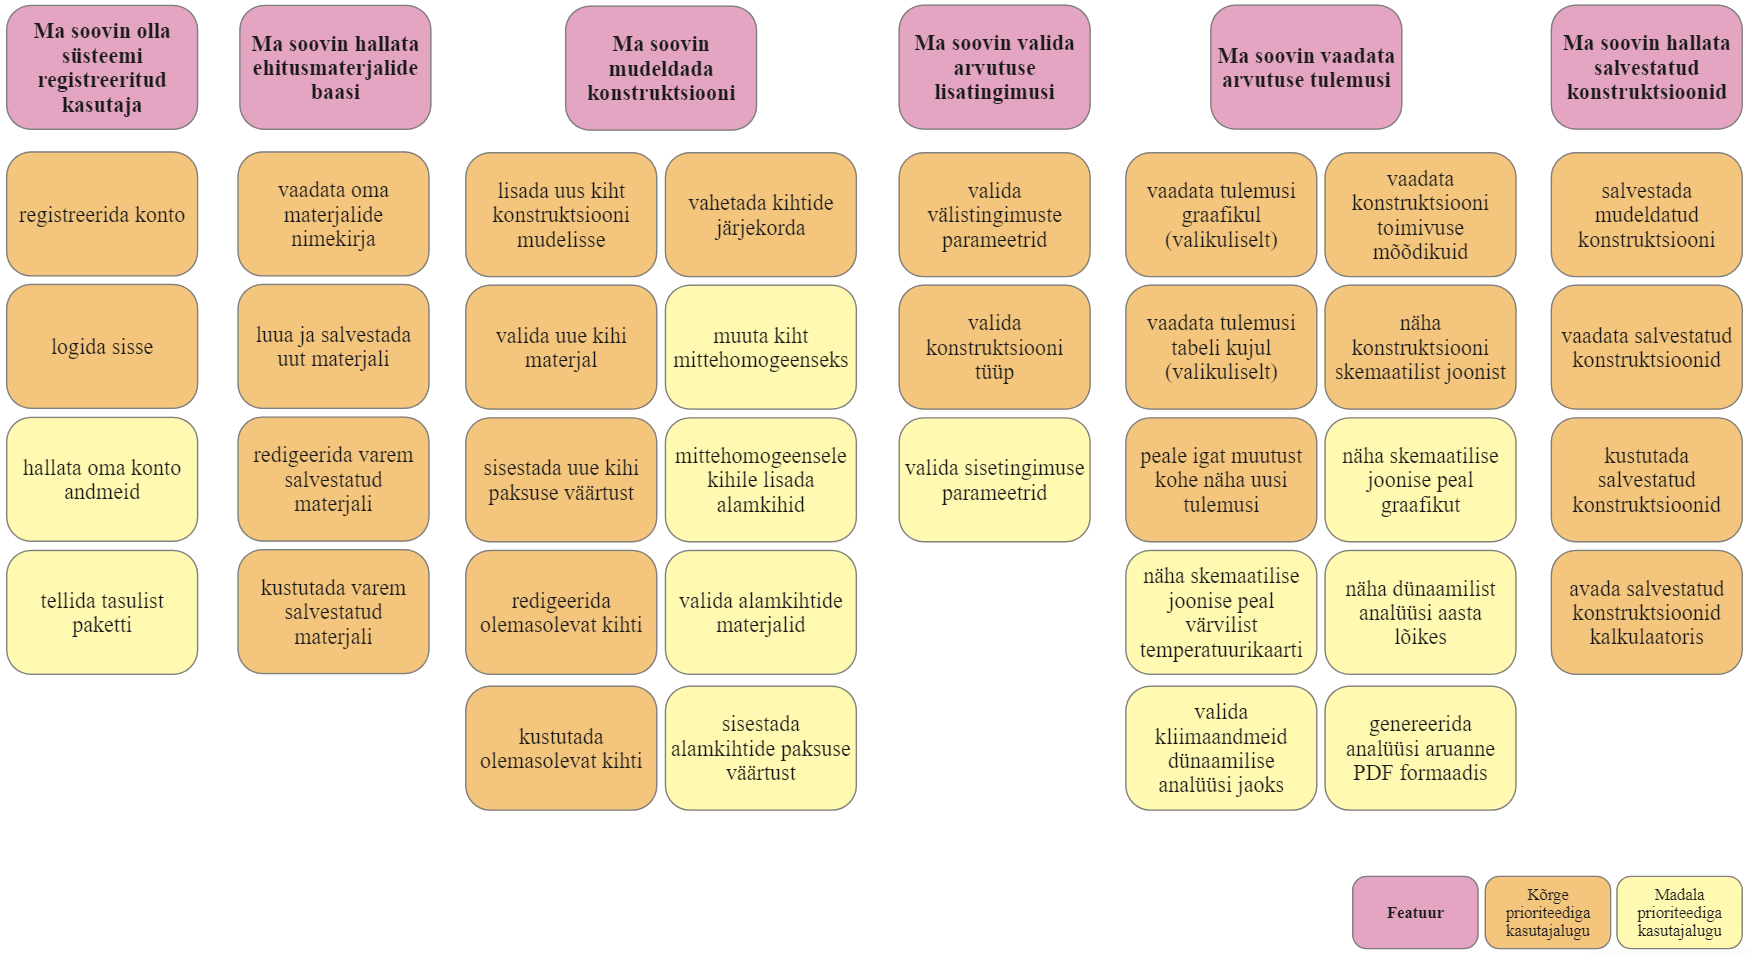
\includegraphics[width=1\textwidth]{figures/analysis/client_userstories.png}
    \caption[Funktsionaalsed nõuded, kliendi kasutajalood]{\textit{Kliendi kasutajalood}}
    \label{fig:client_userstories}
\end{figure}

\begin{figure}[ht]
    \centering
    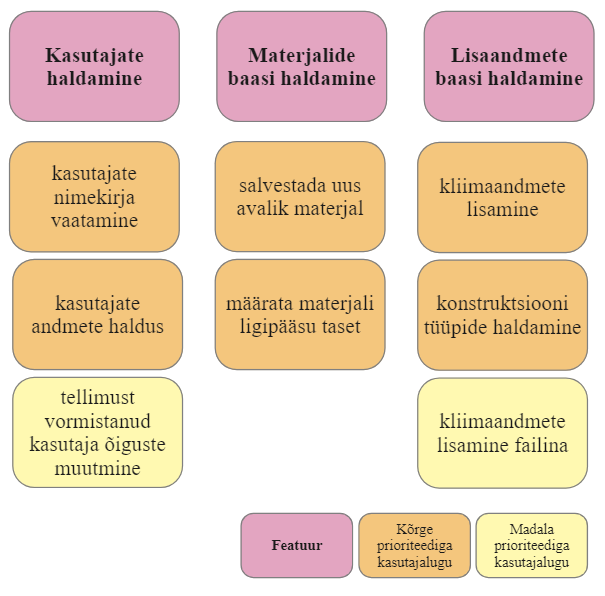
\includegraphics[width=0.6\textwidth]{figures/analysis/admin_userstories.png}
    \caption[Funktsionaalsed nõuded, administraatori kasutajalood]{\textit{administraatori kasutajalood}}
    \label{fig:admin_userstories}
\end{figure}

\subsection{Mittefunktsionaalsed nõuded}
Lisaks osas \ref{subsec_func_req} kirjeldatud funktsionaalsetele nõuetele, peab süsteem vastama järgmistele nõuetele:
\begin{itemize}
    \item kasutajaliides peab olema kiire -- kasutaja peab nägema arvutuse tulemuste uuendamist kohe peale 
lähteandmete (kihid, parameetrid) muutmist, pikk ooteaeg või lehe ümberlaadimine tulemuste näitamiseks ei ole aktsepteeritav;
    \item kasutajaliides peab olema kasutajasõbralik -- kasutaja peab intuitiivselt aru saama, mida ta peaks tegema, et 
jõuda tulemuseni, vajadusel peab ta olema juhitud \textit{popup}-tüüpi infoplokidega;
    \item kasutajaliides peab olema kaasaaegne, st välimus ja veebilehe struktuur peavad
vastama kaasaaegsetele UX/UI printsiibidele.
\end{itemize}
